\chapter[Referencial Teórico]{Referencial Teórico}
\label{chap:referencialTeorico}

Neste capítulo, serão apresentados os conceitos teóricos utilizados como base para o desenvolvimento do Catálogo de Segurança para o Padrão Arquitetural MVC.

Antes mesmo de apresentar os conceitos relevantes para o desenvolvimento do catálogo, é importante entender a definição de software. Este, segundo \cite{sommerville2003engenharia}, pode ser entendido como programas de computador e toda documentação associada. Para realização do desenvolvimento de um software, considerando as boas práticas da área, existem preocupações que merecem menção, sendo essas estabelecidas pela comunidade da Engenharia de Software, incluindo aspectos inerentes à produção \cite{sommerville2003engenharia}. A Figura \ref{BigPicture} apresenta o escopo de atuação desse trabalho, partindo da Engenharia de Software e apoiando-se, principalmente, em duas disciplinas: 

\begin{itemize}
	
	\item Engenharia de Requisitos, que estabelece um conjunto de tarefas e técnicas que auxiliam a promoção do entendimento dos requisitos, sendo uma disciplina detalhada na seção \ref{sec:requisitos}. Será observado que esse trabalho concentra-se em uma abordagem orientada à meta. Portanto, tem-se a Engenharia de Requisitos Orientada à Meta. Essa abordagem trata os requisitos como metas a serem alcançadas, sendo esse estudo apresentado na subseção \ref{subsec:orientacaoMeta}. Especificando ainda mais a área de atuação, como esse trabalho centraliza seus esforços nos RNFs, em particular para elaboração do catálogo, a subseção \ref{subsec:requisitosNaoFuncionais} define conceitos associados aos RNFs, preparando o leitor para a apresentação de um \textit{framework} conceitual especificamente proposto para detalhamento de RNFs. Trata-se do NFR \textit{Framework}, o qual será acordado na seção \ref{sec:NFR}, e
	
	\item Desenho de Software, que se preocupa, dentre outras atividades, com o planejamento e a definição da Arquitetura de Software utilizada. Para fins desse trabalho, o foco será no Padrão Arquitetural MVC. Conceitos associados à Arquitetura de Software bem como ao Padrão Arquitetural MVC serão detalhados na seção \ref{sec:arquitetura} e não subseção \ref{subsec:mvc}, respectivamente.
	
\end{itemize}

\pagebreak

\begin{figure}[h!]
	\centering
	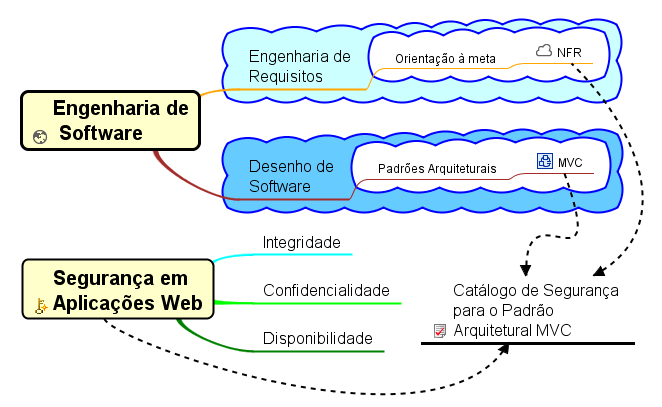
\includegraphics[keepaspectratio=true,scale=0.8]{figuras/bigPicture.png}
	\caption{Áreas de atuação do presente trabalho e conceitos associados.}
	\label{BigPicture}
\end{figure}

Cabe ressaltar que o presente trabalho atua mais especificamente no requisito não funcional Segurança, dada a sua relevância, conforme pesquisa na literatura. Segundo \cite{chung2012non}, Segurança pode ser entendida como a satisfação de três conceitos: Integridade, Confidencialidade, e Disponibilidade. Portanto, o Catálogo de Segurança parte desses conceitos, seguindo a expressão \ref{eq:EstruturaLogicaDeSeguranca}. Segurança, sobre a ótica de um RNF, será tratada na seção \ref{sec:seguranca}. Por fim, visando apoiar a elaboração bem como a documentação dos cenários de uso para aplicação do Catálogo de Segurança, foi utilizado o conceito de personas, o qual será tratado na seção \ref{sec:personas}.

\begin{equation}
	\label{eq:EstruturaLogicaDeSeguranca}
	\textrm{Integridade E Confidencialidade E Disponibilidade SATISFAZ Segurança}
\end{equation}

\section{Engenharia de Requisitos}
\label{sec:requisitos}

Ao conjunto de tarefas e técnicas utilizadas para promover o entendimento dos requisitos é denominado Engenharia de Requisitos \cite{pressman2011engenharia}. No desenvolvimento de software, ela pode ser vista como uma disciplina importante da Engenharia de Software, que se inicia nas atividades de comunicação com os \textit{stakeholders}, e continua até a entrega do produto, sendo adaptada de acordo com as necessidades do processo de desenvolvimento, do produto e dos \textit{stakeholders} \cite{pressman2011engenharia}.

A Engenharia de Requisitos abrange sete fases distintas: concepção, levantamento, elaboração, negociação, especificação, verificação e validação \cite{pressman2011engenharia}. De acordo com \cite{kotonya1998requirements}, durante a execução das atividades nas fases da Engenharia de Requisitos, alguns problemas são relatados como: (i) os requisitos não refletem as reais necessidades do cliente, de acordo com o sistema a ser desenvolvido; (ii) os requisitos são inconsistentes e/ou incompletos; (iii) a Engenharia de Requisitos é complexa e possui alto custo, principalmente, quando há necessidade de mudanças após os requisitos serem ditos acordados/elicitados entre as partes; e (iv) os requisitos são comumente interpretados de maneira errada pela equipe de desenvolvimento, diante do que foi solicitado pelo cliente. Apesar de parecer algo acordado em uma referência antiga da área. Tais problemas continuam ocorrendo em desenvolvimentos atuais, conforme apontado em palestras recentes de autores da área \cite{palestrasilvio}. 

Boa parte dos modelos utilizados na Engenharia de Requisitos não possuem tratamento adequado para lidar com os critérios de qualidade. Logo, o tratamento desses critérios tem sido uma preocupação para a comunidade da Engenharia de Requisitos. Atualmente, existem esforços no sentido de aprimorar os modelos e as especificações desses requisitos, e são fortemente associados à comunidade de pesquisadores da Engenharia de Requisitos Orientada à Meta (GORE) \cite{chung2012non}. Neste trabalho, é abordado o uso de uma notação específica para tratar RNFs, proposta por essa comunidade, no caso, trata-se do NFR \textit{framework} \cite{chung2012non}. 

O NFR \textit{framework} é um \textit{Framework} conceitual que procura lidar com os requisitos não funcionais, permitindo especificar os mesmos em um alto nível de abstração e, gradualmente, fornecendo insumos para que essa especificação seja trazida para um nível mais baixo de abstração. Nesse último nível, são especificadas as operacionalizações, as quais evidenciam alternativas para viabilizar a implementação desses requisitos no nível de código. Mais adiante, serão apresentados detalhes dessa notação.

\subsection{Engenharia de Requisitos Orientada à Meta}
\label{subsec:orientacaoMeta}

A Engenharia de Requisitos Orientada à Meta (GORE) tem-se popularizado nos últimos anos e foca seus esforços no tratamento dos requisitos, como metas a serem alcançadas \cite{van2001goal}. Seus modelos possuem como objetivo a modelagem da razão pela qual determinado requisito existe. Essa modelagem promove ao Engenheiro de Requisitos uma estratégia mais detalhada do problema, podendo encontrar uma solução mais adequada \cite{van2001goal}\cite{chung2012non}. O GORE é uma abordagem cada vez mais reconhecida na comunidade de Engenharia de Requisitos \cite{van2001goal}.

Nas definições do GORE, existem as metas que são componentes essenciais. De acordo com \cite{van2001goal}, uma meta é definida como uma propriedade do sistema, a qual é expressa pelos \textit{stakeholders} através de determinadas questões como: “\textbf{Porquê}” uma meta é exigida, “\textbf{como}” ela pode ser atingida, e “\textbf{quem}” será o responsável pela meta no sistema e no ambiente.

\begin{figure}[h!]
	\centering
	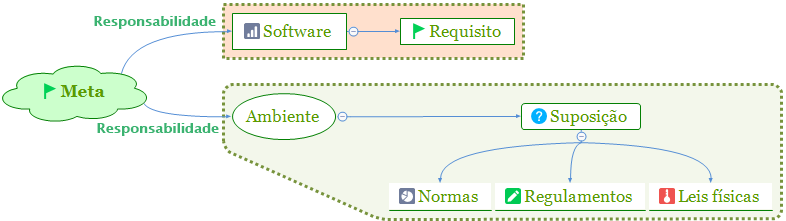
\includegraphics[keepaspectratio=true,scale=0.8]{figuras/GORE.png}
	\caption{Responsabilidades da meta sob o software e sob o ambiente.}
	\label{Gore}
\end{figure}


\pagebreak

 Com base na Figura \ref{Gore}, pode-se entender como são os comportamentos das metas na abordagem GORE. Representada pelo símbolo de uma nuvem, uma meta, quando está sob a responsabilidade de um único software, pode se tornar um requisito. De forma semelhante, quando uma meta está sob a responsabilidade de um ambiente, ela pode se tornar uma suposição. Diferentemente de um requisito, uma suposição não pode ser aplicada pelo software. Mas, pode ser satisfeita devidos às normas, aos regulamentos organizacionais e às leis físicas\cite{van2001goal}. Esse trabalho focou apenas nas responsabilidades voltadas ao software.

\begin{comment}
	Existem diversos \textit{frameworks} orientados à meta. Os principais  são o NFR \textit{Framework} \cite{chung2012non} e o i* \cite{istarwiki20}. Ambos esses \textit{frameworks} serão detalhados nas seções \ref{sec:NFR} e \ref{sec:i*}, respectivamente.
\end{comment}


\subsection{Requisitos Não-Funcionais}
\label{subsec:requisitosNaoFuncionais}

A visão do software como um produto fez com que os aspectos que avaliam a qualidade de um software passassem a possuir maior atenção. Apenas satisfazer requisitos funcionais não é o suficiente. Logo, tem-se maior atenção para o RNFs, tais como: Segurança, Integridade, Disponibilidade, dentre outros \cite{cysneiros1997definindo}.

Os RNFs podem ser entendidos como restrições sobre como os requisitos funcionais devem ser implementados, e determinam como o software deve realizar suas funções \cite{sommerville1997requirements}.


Júlio Leite, afirma em sua pesquisa que os RNFs impactam o produto software em qualidade e preço, pois segundo ele:

\begin{citacao}
	“A não observância da necessidade de RNFs durante o processo de desenvolvimento do software, pode levar uma recodificação custosa e demorada o que consequentemente, eleva o preço do software.” \cite[p. 2]{cysneiros1997definindo}
\end{citacao}


Os RNFs devem ser analisados em toda sua magnitude para o desenvolvimento e a manutenção de um produto de software, sendo importante analisar os possíveis conflitos que podem ser gerados com outros RNFs bem como com os requisitos funcionais. Esses conflitos, uma vez não identificados em uma fase inicial do processo de desenvolvimento de software, podem acarretar em problemas futuros, durante as atividades de implementação e implantação do software \cite{cysneiros1997definindo}. 


As classes de NFRs \cite{eckhardt2016non} podem ser compreendidas como subtipos dos atributos de qualidade da Tabela \ref{AtributosDeQualidade}, na qual são definidos de acordo com a \cite{organizacion2011iso}. 

\begin{table}[h!]
	\centering
	\caption{Descrição dos atributos de qualidade. Fonte: \cite{organizacion2011iso}.}
	\label{AtributosDeQualidade}
	\begin{tabular}{@{}cc@{}}
		\toprule
		\textbf{\begin{tabular}[c]{@{}c@{}}Atributos de \\ qualidade\end{tabular}} & \textbf{Descrição} \\ \midrule
		Funcionalidade & \begin{tabular}[c]{@{}c@{}}É a capacidade do software de promover funções que\\ atendam às necessidades explícitas e implícitas.\end{tabular} \\
		\rowcolor[HTML]{C0C0C0} 
		Segurança & \begin{tabular}[c]{@{}c@{}}É a capacidade do software de apresentar níveis\\  aceitáveis e riscos de danos a pessoas, negócios\\  software, propriedades ou ambiente.\end{tabular} \\
		Confiabilidade & \begin{tabular}[c]{@{}c@{}}É a capacidade do software de manter o nível de\\ desempenho especificado.\end{tabular} \\
		\rowcolor[HTML]{C0C0C0} 
		Usabilidade & \begin{tabular}[c]{@{}c@{}}É a capacidade do software de ser compreendido,\\ de fácil aprendizagem, operável e atraente ao usuário.\end{tabular} \\
		Eficiência & \begin{tabular}[c]{@{}c@{}}É a capacidade software de apresentar desempenho\\ apropriado, relativo aos recursos utilizados.\end{tabular} \\
		\rowcolor[HTML]{C0C0C0} 
		Portabilidade & \begin{tabular}[c]{@{}c@{}}É a capacidade software de ser transferido de\\ um ambiente para o outro.\end{tabular} \\
		Manutenção & \begin{tabular}[c]{@{}c@{}}É a capacidade do software de modificado de forma\\ eficiente e eficaz.\end{tabular} \\ \bottomrule
	\end{tabular}
\end{table}

\section{NFR Framework}
\label{sec:NFR}

O NFR \textit{Framework}  é um modelo intencional, criado para ajudar os especialistas a lidarem com requisitos não-funcionais, através de um grafo chamado de \textit{Softgoal Interdependency Graphs} (SIGs). Neste tipo de grafo, os requisitos podem ser analisados, uma vez que o SIG permite uma visão vertical desde a estratégia de alto nível até os detalhes operacionais;  possuindo operadores lógicos AND (E) e OR (OU) que promovem uma melhor tomada de decisão. Os RNFs são escritos através de uma notação formal. Essa notação permite comprovar a precisão e a completude de cada NFR \cite{chung2012non}. 

O \textit{framework} também pode ser orientado por processo, dado seu suporte às atividades e fases do processo de Engenharia de Requisitos. Nesse caso, sendo utilizado como complemento nas abordagens de desenvolvimento de software \cite{chung2012non}.

O NFR \textit{Framework} utiliza o conceito de metas  flexíveis. Por definição, uma meta flexível é uma condição ou um estado no mundo real que deseja ser alcançado, podendo assumir natureza subjetiva, uma vez que o RNF pode variar de acordo com o julgamento de cada pessoa; e natureza relativa, uma vez que o RNF pode depender de algum tipo de relação com outro RNF \cite{chung2012non}.

A notação no SIG para a \textbf{meta flexível} é um símbolo similar ao de uma nuvem, conforme apresentado pela Figura \ref{fig01}. Esse símbolo possui pequenas variações na forma, podendo representar uma \textbf{operacionalização} (nuvem em negrito), e também uma \textbf{Alegação} (nuvem tracejada). Mais adiante, na Figura \ref{exemploNFR}, é apresentada a decomposição de uma meta flexível em outras metas.  

\begin{figure}[h!]
	\centering
	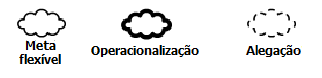
\includegraphics[keepaspectratio=true,scale=0.9]{figuras/elementosSIG.png}
	\caption{Representações gráficas de Meta Flexível, Operacionalização e Alegação.}
	\label{fig01}
\end{figure} 

Para facilitar o entendimento das decisões tomadas, a meta flexível possui \textit{labels}, que determinam o grau de satisfação para uma meta flexível, de acordo com um conjunto de decisões do projeto. As \textit{labels} são: satisfeita, fracamente satisfeita,  negada, fracamente negada, indecidida e crítica \cite{chung2012non}. Outra notação importante, e que apresenta o grau de prioridade de uma meta flexível, é representada por “\textbf{!}” ou “\textbf{!!}” permitindo especificar um grau de prioridade maior, sendo o ponto de afirmação desenhado à esquerda da nuvem..

\begin{figure}[h]
	\centering
	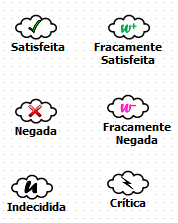
\includegraphics[keepaspectratio=true,scale=0.9]{figuras/labelsSoftgoals.png}
	\caption{Representação gráfica das \textit{labels} em metas flexíveis.}
	\label{fig02}
\end{figure} 

As relações que as metas flexíveis possuem umas com as outras são estabelecidas através de \textit{links} de interdependências, sendo esses \textit{links} que realizam o registro da decomposição das metas flexíveis em metas flexíveis mais específicas (filhos). De certa forma, a decomposição em outras metas contribui para o nível de satisfação da meta flexível mais genérica (pai).

Os \textit{links} de interdependências também podem ser entendidos como tipos de contribuições, e possuem uma notação simbólica para cada tipo, e cada tipo possui ainda um significado.  Tais tipos de contribuição são apresentados na Tabela \ref{tiposDeContribuições}, adaptados de  \cite{chung2012non}.



\begin{table}[h!]
	\centering
	\caption{Tipos de contribuições.}
	\label{tiposDeContribuições}
	\begin{tabular}{@{}cl@{}}
		\hline
		\textbf{Símbolo} & \textbf{Descrição} \\ \hline
		\multirow{2}{*}{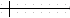
\includegraphics[scale=0.9]{figuras/And.png}} & \multirow{2}{*}{AND: Se todos os filhos são satisfeitos, o pai também será satisfeito.} \\
		&  \\ \hline
		\multirow{2}{*}{\includegraphics[scale=0.9]{figuras/OR.png}} & \multirow{2}{*}{OR: Se qualquer filho é satisfeito, o pai também será satisfeito.} \\
		&  \\ \hline
		\multirow{2}{*}{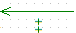
\includegraphics[scale=0.9]{figuras/Make.png}} & \multirow{2}{*}{\begin{tabular}[c]{@{}l@{}}MAKE: Pode ser tratado de forma semelhante ao AND, pois, se \\ o filho for satisfeito, o pai pode ser satisfeito.\end{tabular}} \\
		&  \\ \hline
		\multirow{2}{*}{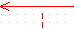
\includegraphics[scale=0.9]{figuras/Break.png}} & \multirow{2}{*}{\begin{tabular}[c]{@{}l@{}}BREAK: Fornece apoio negativo, pois, se o filho é satisfeito, o \\ pai pode ser negado.\end{tabular}} \\
		&  \\ \hline
		\multirow{2}{*}{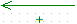
\includegraphics[scale=0.9]{figuras/Help.png}} & \multirow{2}{*}{HELP: Se todos os filhos são satisfeitos, o pai também será satisfeito.} \\
		&  \\ \hline
		\multirow{2}{*}{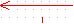
\includegraphics[scale=0.9]{figuras/Hurt.png}} & \multirow{2}{*}{HURT: Se todos os filhos são satisfeitos, o pai será fracamente negado.} \\
		&  \\ \hline
		\multirow{2}{*}{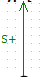
\includegraphics[scale=0.9]{figuras/SomeMais.png}} & \multirow{2}{*}{SOME+: Representa a existência de alguma contribuição positiva.} \\
		&  \\ \hline
		\multirow{2}{*}{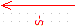
\includegraphics[scale=0.9]{figuras/SomeMenos.png}} & \multirow{2}{*}{SOME-: Representa a existência de alguma contribuição negativa.} \\
		&  \\ \hline
	\end{tabular}
\end{table}

\pagebreak

Os \textit{links} entre as metas flexíveis representam a contribuição que uma meta flexível tem com outra meta flexível, ou operacionalização, ou alegação. Logo, a Figura \ref{catalogoDeAvaliação} apresenta a forma como as \textit{labels} são propagadas, de acordo com seu tipo de relacionamento. A propagação das \textit{labels} aplica-se a todos os tipos de representações da notação, sendo essas: metas flexíveis, operacionalizações ou alegações.. 

\begin{figure}[h!]
	\centering
	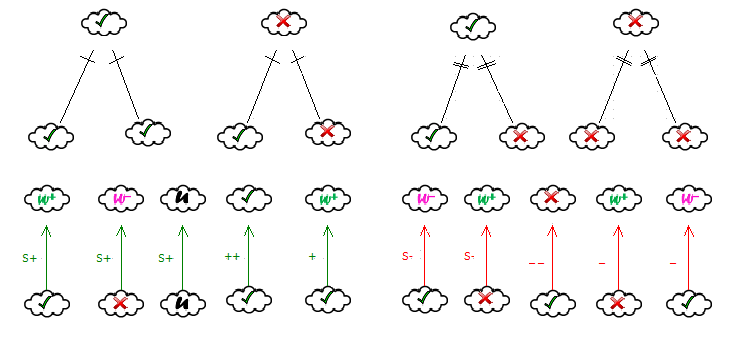
\includegraphics[keepaspectratio=true,scale=0.8]{figuras/catalogoDeAvaliacao.png}
	\caption{Propagação das \textit{labels} para os diferentes tipos de contribuição. Adaptado de \cite{chung2012non}.}
	\label{catalogoDeAvaliação}
\end{figure} 

\pagebreak

A Figura \ref{exemploNFR} apresenta uma decomposição de uma meta flexível em diferentes níveis de abstração. Consideramos, nesse exemplo, o RNF: “manter as contas com boa segurança”. Usando a notação do NFR \textit{Framework}, representou-se a meta flexível  “segurança de contas”, no nível mais generalista do grafo. Em segundo nível, são especificadas as principais metas flexíveis que merecem ser consideradas para que a meta generalista seja "satisfeita", no caso: “Integridade de contas”, “Confidencialidade de contas” e “Disponibilidade de contas” \cite{chung2012non}.

\begin{figure}[h!]
	\centering
	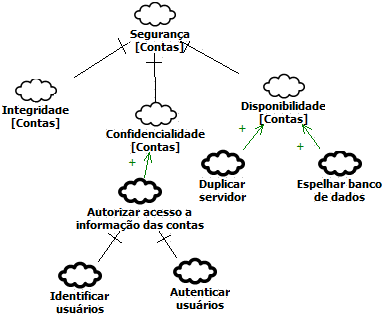
\includegraphics[keepaspectratio=true,scale=1.0]{figuras/exemploNFR.png}
	\caption{Operacionalização de segurança de contas. Adapatado de \cite{chung2012non}, \cite{affleck2012supporting}.}
	\label{exemploNFR}
\end{figure} 

Confidencialidade de contas é operacionalizada em ``Autorizar acesso à informação das contas``, que possui uma contribuição do tipo HELP com seu pai. Dada a relação do tipo AND, entre essa operacionalização e as operacionalizações ``Identificar usuários`` e ``Autenticar usuários``, tem-se que a operacionalização ``Autorizar acesso à informação das contas``  será realizada, se ambas as operacionalizações, ``Identificar usuários`` e ``Autenticar usuários``, forem realizadas. Supondo que tudo tenha sido realizado com sucesso, tem-se que esse processo de operacionalização contribui positivamente - HELP (AJUDA) - a atingir ``Confiabilidade de contas``. Como essa meta flexível está especificada em uma relação de AND com as metas flexíveis "Integridade de contas" e ``Disponibilidade de contas``, pode-se dizer que em termos de ``Confiabilidade de contas``, ``Segurança de contas`` tende a ser ``satisfeita``. Mas, resta ainda ponderar se "Integridade de contas" e ``Disponibilidade de contas`` serão de fato ``satisfeitas``. O modelo, da forma como está especificado, não permite avaliar tais aspectos, visto que representa apenas uma visão parcial dessas metas flexíveis.


Para Disponibilidade de contas, a mesma é operacionalizada em “Duplicar servidor” e “Espelhar banco de dados”. Essas operacionalizações possuem contribuições do tipo HELP e mesmo pai. Para a meta flexível ser satisfeita, ambas as operacionalizações devem ser satisfeitas \cite{affleck2012supporting}. 


\begin{comment}


\section{Framework i*}
\label{sec:i*}


Outra abordagem orientada à meta, o \textit{framework} de modelagem i*\footnote[1]{O nome i* faz referência a utilização da notação de distribuição intencional que é a base do \textit{framework}.}, possui foco em ambientes organizacionais e seus sistemas de informação, tomando como base os relacionamentos de dependência entre os atores participantes \cite{yu1997towards} \cite{istarwiki20}. 

O \textit{framework} é composto por dois modelos: o (i) Modelo de Dependência Estratégica (do inglês, \textit{Strategic Dependency - (SD)}), utilizado para descrever as relações de dependência entre vários atores em um contexto organizacional, e o (ii) Modelo de Razão estratégica (do inglês, \textit{Strategic Rationale - (SR)}), utilizado para descrever os interesses e preocupações das partes interessadas, e como eles podem ser abordados pelas configurações do ambiente e dos sistemas \cite{yu1997towards}. Esses dois modelos serão detalhados a seguir, nas subseções \ref{subsec:SD} e \ref{subsec:SR}.

Com a utilização do \textit{framework}, é possível representar, por meio de seus modelos, os atores participantes e suas dependências, para que suas metas sejam alcançadas, recursos fornecidos, tarefas realizadas e metas flexíveis sejam “satisfeitas a contento” ou “razoavelmente satisfeitas” \cite{istarwiki20}.
 
 
\subsection{Modelo de Dependência Estratégica - SD}
\label{subsec:SD}

O modelo SD é utilizado para expressar, através de uma rede de relacionamentos estratégicos e intencionais, a relação entre os atores em um contexto organizacional. Em sua modelagem, o modelo utiliza um conjunto de nós e ligações. Cada nó representa um ator, e cada ligação entre dois atores indica que um determinado ator depende de outro, para que um objetivo possa ser atingido \cite{istarwiki20}. Os atores e suas dependências podem ser representados de acordo com os símbolos das Figuras  \ref{atoresIstar} e \ref{dependenciaIstar}.

\begin{figure}[h!]
	\centering
	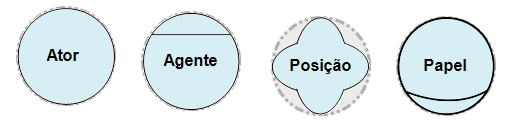
\includegraphics[keepaspectratio=true,scale=1.0]{figuras/papeisIstar.PNG}
	\caption{Símbolos que representam atores no i*.}
	\label{atoresIstar}
\end{figure}

De acordo com as definições de \cite{istarwiki20}, um  \textbf{Ator} é o termo utilizado para referir de forma genérica a qualquer unidade em que as dependências intencionais possam ser atribuídas. Os agentes, as posições e os papeis podem ser entendidos como subunidades de um ator mais complexo e sendo definidas como: 

\begin{itemize}
	\item \textbf{Agente}: Ator, normalmente quando automatizado, em algum contexto específico;
	 
	\item \textbf{Posição}: É definido como um conjunto de funções desempenhadas por um agente, também compreendido como uma abstração intermediária entre um Papel, um Agente ou Ator, sendo possível dizer que se um Agente ou Ator ocupa uma Posição, essa Posição cobre um Papel;
	
	\item \textbf{Papel}: É definido como manifestações concretas e físicas, utilizado para se referir a Atores e Agentes de \textit{Hardware}/\textit{Software}.
\end{itemize} 

No modelo Dependência Estratégica, ao existir uma cooperação entre dois atores, essa cooperação é denominada de dependência, na qual existe um ``dependente`` (\textit{depender}) e um ``de quem se depende`` (\textit{dependee}). Esses atores, \textit{depender} e \textit{dependee}, são ligados por um elo de dependência (\textit{dependum}), que pode ser uma meta a ser atingida, uma tarefa a ser realizada, um recurso a ser fornecido ou uma meta flexível a ser razoavelmente satisfeita \cite{napolitano2009estrategia}. 

\begin{figure}[h!]
	\centering
	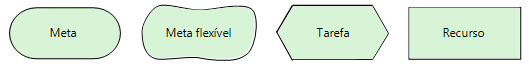
\includegraphics[keepaspectratio=true,scale=1.0]{figuras/TiposDeContribuicao.png}
	\caption{Símbolos que representam o elo de dependência.}
	\label{dependenciaIstar}
\end{figure} 

Os tipos de dependências são definidos por \cite{istarwiki20} como: 

\begin{itemize}
	
	\item \textbf{Meta}: Uma condição ou estado de desejo intencional do ator no mundo real. Os detalhes de como a meta deve ser satisfeita não são descritos, promovendo então a decomposição da mesma em uma série de alternativas.  
	 
	\item \textbf{Meta flexível}: De maneira semelhante à Meta, também representa uma condição ou estado de desejo intencional do ator no mundo real. Entretanto, os detalhes de como a meta flexível deve ser satisfeita não são definidos a princípio, sendo então sujeitos a interpretação. Para verificar se uma meta flexível foi satisfeita, utiliza-se os termos ``satisfeita a contento`` ou ``razoavelmente satisfeita``, pois metas flexíveis não possuem critérios claramente definidos. 
	
	\item \textbf{Tarefa}: Representa a realização de algo em forma particular por um ator. Uma tarefa também pode ser decomposta em subtarefas mais específicas. 
	
	\item \textbf{Recurso}: Representa uma entidade física ou informativa, pressupõe-se, então, que não existe nenhum problema ou questões abertas sobre como a recurso será alcançado.
	 
\end{itemize}

A partir das definições dos tipos de dependência e dos atores é possível modelar a relação de dependência entre dois ou mais atores. Como apresentado no exemplo da Figura \ref{exemploTipoDeDepencia}, na qual, na modelagem, existem dois atores, \textbf{Titular do cartão}, e \textbf{Banco}, sendo possível perceber a existência dos quatro tipos de dependência: dependência por recurso, dependência por tarefa, dependência por meta flexível e dependência por meta.  

\begin{figure}[h!]
	\centering
	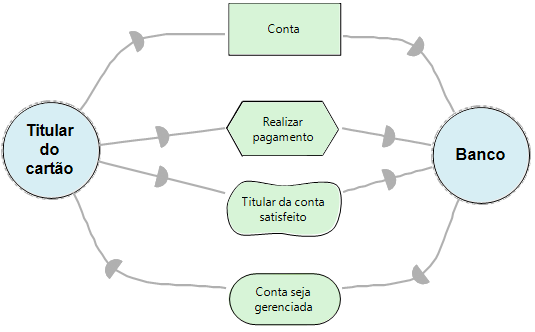
\includegraphics[keepaspectratio=true,scale=1.0]{figuras/ExemploTiposDeDependecias.PNG}
	\caption{Exemplo dos tipos de dependência entre o Títular do cartão e o Banco.}
	\label{exemploTipoDeDepencia}
\end{figure} 

\begin{itemize}
	
	\item \textbf{Dependência por recurso}: Neste tipo de dependência, o \textit{depender} depende do \textit{dependee} para que ocorra a disponibilidade do recurso. Ao determinar essa dependência, o \textit{depender} pode utilizar a entidade como um recurso \cite{istarwiki20}. No contexto da figura \ref{exemploTipoDeDepencia}, esse elo existe através do recurso \textbf{Conta}. O \textbf{Títular do cartão} é o \textit{depender}, ou seja, possui uma relação de dependência com o \textbf{Banco} (\textit{dependee}) para que o recurso, \textbf{Conta}, seja fornecido.
	
	\item \textbf{Dependência por tarefa}: Neste tipo de dependência, o \textit{depender} depende do \textit{dependee} para realização da tarefa. A tarefa pode ser entendida como uma restrição imposta pelo \textit{depender} ao \textit{dependee}, na qual o \textit{dependee} possui certa liberdade de ação dentro dessas restrições \cite{istarwiki20}. No contexto da Figura \ref{exemploTipoDeDepencia}, esse elo existe através da tarefa \textbf{Realizar pagamento}, onde o \textbf{Títular do cartão} é o \textit{depender}. Esse último depende da disponibilização do \textbf{Banco} para \textbf{Realizar pagamento} ao \textbf{Banco}. 
	
	\item \textbf{Dependência por meta flexível}: Neste tipo de dependência, o \textit{depender} depende do \textit{dependee} para que alguma tarefa seja realizada para que a meta flexível possa ser ``satisfeita a contento`` ou ``razoavelmente satisfeita`` \cite{istarwiki20}. O \textit{depender} determina se a meta flexível será alcançada ou não utilizando as habilidades e conhecimentos do \textit{dependee} \cite{napolitano2009estrategia}. No contexto da Figura \ref{exemploTipoDeDepencia}, esse elo existe através da meta flexível \textbf{Titular da conta satisfeito}. Nesse caso, o \textbf{Títular do cartão} é o \textit{depender}. Ele depende da forma como o serviço do \textbf{Banco} é prestado para que o \textit{depender} possa decidir se a meta flexível será alcançada.
	
	\item \textbf{Dependência por meta}: Neste tipo de dependência, o \textit{depender} depente do \textit{dependee} para que um estado no mundo real seja alcançado. O \textit{dependee} possui total liberdade para tomar as decisões necessárias para atingir a meta. O \textit{depender} não se preocupa com o quanto o \textit{dependee} destina-se em satisfazer a meta \cite{istarwiki20}. No contexto da Figura \ref{exemploTipoDeDepencia}, esse elo existe através da meta \textbf{Conta seja gerenciada},  \textbf{Banco} é o \textit{depender}, pois, espera-se que o \textbf{Títular do cartão} tenha capacidade de gerir sua própria conta, através dos recursos fornecidos pelo \textbf{Banco}. 
	
\end{itemize}

\subsection{Modelo de Razão Estratégica - SR}
\label{subsec:SR}

O modelo SR apresenta de forma gráfica, com vários tipos de nós (Meta, Tarefa, Recurso e Meta flexível)\footnote[1]{Os tipos de nós possuem as mesmas definições que os tipos de dependências no Modelo de Dependência Estratégica (SD) descritos na Subseção \ref{subsec:SD}} e links (links de meio-fim, links de decomposição de tarefas e links de contribuição), os quais servem como estrutura representacional que expressam as razões por trás das dependências \cite{istarwiki20}.

O modelo tem o objetivo principal de representar, de forma detalhada, as estratégias internas dos atores em função dos elementos do processo, das alternativas e das decisões por trás do processo, Essas estratégias internas dos atores representam como as metas são alcançadas, os recursos são disponibilizados, e as metas flexíveis são refinadas e operacionalizadas \cite{napolitano2009estrategia}.  

De acordo com \cite{istarwiki20}, os tipos de \textit{links} são definidos como: 

\pagebreak

\begin{itemize}
	
	\item \textbf{\textit{link} de meio-fim}: Representado graficamente por uma seta direcionada para o nó fim. O ``\textbf{meio}`` normalmente é expresso por uma tarefa, que define o ``como`` fazer algo. O " \textbf{fim}`` expressa à meta a ser alcançada.
\end{itemize}

\begin{figure}[h!]
	\centering
	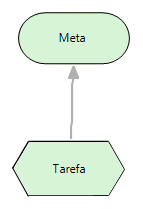
\includegraphics[keepaspectratio=true,scale=0.9]{figuras/meioFim.PNG}
	\caption{Notação gráfica para o \textit{link} de meio-fim. Adaptado de \cite{istarwiki20}.}
	\label{meiofim}
\end{figure} 

\begin{itemize}	
	\item \textbf{\textit{link} de decomposição}: Uma tarefa pode ser decomposta em submeta, subtarefa, recurso ou meta flexível. A representação gráfica para um \textit{link} de decomposição é um segmento de reta com um pequeno corte perpendicular, como apresentado na Figura \ref{decomposicaoLink}.    
\end{itemize}	

\begin{figure}[h!]
		\centering
		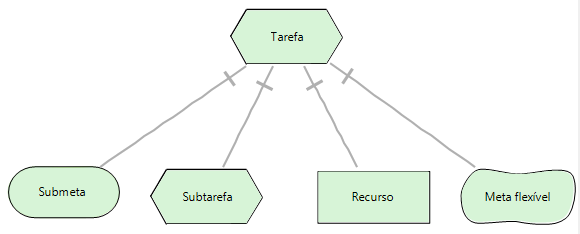
\includegraphics[keepaspectratio=true,scale=1.0]{figuras/decomposicaoLink.PNG}
		\caption{Notação gráfica para o \textit{link} de decomposição. Adaptado de \cite{istarwiki20}.}
		\label{decomposicaoLink}
\end{figure}

\begin{itemize}		
	\item \textbf{\textit{links} de contribuição}: Os tipos de contribuições\footnote[1]{A definição de cada tipo de contribuição é a mesma dada por Chung em \cite{chung2012non}, como visto na Tabela \ref{tiposDeContribuições}, que detalha os tipos de contribuições para o NFR Framework.} entre as metas flexíveis são: \textit{Make}, \textit{Some+}, \textit{Help}, \textit{Unknown}, \textit{Break}, \textit{Some-}, \textit{Hurt}, \textit{Or} e \textit{And}. 
\end{itemize}
\end{comment}

A comunidade científica dedicada à abordagem GORE, conforme exposto nas últimas seções, centraliza seus esforços e contribuições na especificação de metas flexíveis, com modelos que detalham essa especificação em diferentes níveis de abstração. Entretanto, essa preocupação com os RNFs é ainda mais antiga, visto que temos especificações anteriores às iniciativas orientadas à meta, como é o caso do FURPs. Conforme será notado com a leitura da próxima seção, FURPS tem um rigor na especificação de metas flexíveis muito inferior à notação do NFR e similares adotadas pela comunidade GORE. Diante dessas colocações, e dada a importância dos RNFs para o escopo desse trabalho, justifica-se o uso do NFR \textit{Framework} nesse caso.

\section{FURPS}
\label{sec:furps}

O termo FURPS é um acrônimo que define um modelo de atributo de qualidade. Esse acrônimo é composto por cinco atributos de qualidade, sendo eles: (i) Funcionalidade (do inglês, \textit{Functionality}), (ii) Usabilidade (do inglês, \textit{Usability}), Confiabilidade (do inglês, \textit{Reliability}), Desempenho (do inglês, \textit{Performance}) e \textit{Supportability} (manteve-se o termo em inglês, pois o mesmo significa considerar testabilidade, adaptabilidade, manutenibilidade, compatibilidade, configurabilidade, escalabilidade e outros aspectos associados, não sendo, portanto, possível encontrar um único termo em português capaz de representar todos esses aspectos). \cite{umar2011analyzing}.

\subsection{Funcionalidade}
\label{subsec:funcionalidade}

São os requisitos funcionais de uma aplicação de software. A funcionalidade está diretamente ligada ao comportamento do software e à interação do usuário com o software \cite{cintra2006implementaccao}.

Por definição, funcionalidade é a capacidade do software de promover funções que atendam às necessidades explícitas e implícitas quando o software estiver sendo utilizado, de acordo com os cenários especificados \cite{qualidadeDeProdutoNBR}.

\subsection{Usabilidade}
\label{subsec:usabilidade}

Quando se pensa em usabilidade, tem-se uma preocupação com a satisfação do usuário, levando em conta, por exemplo, sua experiência em manipular um computador, utilizar um software, questões de ergonomia, design da interface gráfica, e até mesmo o contexto para o qual a solução computacional está sendo desenvolvida \cite{cintra2006implementaccao}.

Por definição, usabilidade é a capacidade do software de ser compreendido, aprendido, operado e atraente ao usuário, quando o software estiver sendo utilizado de acordo com os cenários especificados \cite{qualidadeDeProdutoNBR}.


\subsection{Confiabilidade}
\label{subsec:confiabilidade}

No caso da Confiabilidade, considera-se a prevenção de falhas, capacidade do software se recuperar de um erro, a precisão e o tempo entre falhas (\textit{Mean Time Between Failure} (MTBF)) \cite{cintra2006implementaccao}.

Por definição, confiabilidade é a capacidade do software em manter o nível de estabilidade esperado, garantindo, por exemplo, tolerância a falhas e até mesmo recuperação rápida diante da ocorrência dessas falhas, quando o software estiver sendo utilizado de acordo com os cenários especificados \cite{qualidadeDeProdutoNBR}.  

\subsection{Desempenho}
\label{subsec:desempenho}

Em desempenho, são relevantes vários aspectos. Alguns deles, como garantir tempo de recuperação adequado, são necessidades sombreadas e desejadas em outros critérios também, no caso, confiabilidade. Outros aspectos chave, inerentes ao escopo do critério desempenho, são: taxas de transferência e transmissão de dados (do inglês, \textit{troughput})\footnote[1]{Quantidade de dados que pode ser tranferidos de um lugar para o outro em um espaço de tempo previamente especificado.}, e consumo de recursos (energia, memória, processamento, cache, uso balanceado/otimizado do sistema operacional, entre outros \cite{cintra2006implementaccao}.

Por definição, desempenho é o nível como o software atende ao conjunto específico de valores, especificado para cada característica atrelada à execução desse software \cite{qualidadeDeProdutoNBR}.  

\subsection{\textit{Supportability}}
\label{subsec:suportabilidade}

Em \textit{Supportability}, considera-se a capacidade de adaptabilidade, a possibilidade de realizar manutenções corretivas e evolutivas, a flexibilidade de configuração, de instalação e a internacionalização no sistema \cite{cintra2006implementaccao}.

Dado que esse trabalho abrange duas áreas, Engenharia de Requisitos e Arquitetura de Software, e que o maior olhar até o momento foi na primeira área, seguem seções que acordam referenciais associados à Arquitetura de Software. 

\section{Arquitetura de Software}
\label{sec:arquitetura}

O conceito de \textit{design} de software surgiu da década de 1970, quando os pesquisadores da época acreditavam que o \textit{design} era uma atividade separada da implementação, exigindo notações, técnicas e ferramentas específicas. Foi somente a partir da década de 1990 que se utilizou o termo arquitetura de software, em contraste com \textit{design} de software, para indicar noções de codificação, abstrações, padrões e treinamentos formais de arquitetos de software \cite{perry1992foundations}.

O termo arquitetura de software é definido por \cite{shaw1996software}, como o entendimento do sistema em termos de seus componentes computacionais e os relacionamentos entre os componentes, os padrões que guiam a composição organizacional dos componentes, bem como as decisões de restrições arquiteturais. 

As arquiteturas de software são projetadas de acordo com algum princípio de estruturação genérico, sendo esses princípios chamados de padrões arquiteturais \cite{buschmann1996system}. 

Os padrões arquiteturais são modelos para arquiteturas concretas de software, expressando a estrutura essencial para o desenvolvimento de um produto de software. O padrão fornece um conjunto de subsistemas predefinidos, incluindo regras e diretrizes para organizar as relações entre eles, além de especificar suas responsabilidades \cite{buschmann1996system}. 

A seleção de um padrão arquitetural é uma atividade fundamental ao desenvolver um sistema de software, sendo apropriado entender que cada padrão auxilia o desenvolvedor a alcançar uma propriedade de sistema específica. Dentre o conjunto dos padrões arquiteturais, existem padrões que auxiliam em propriedades similares, e podem ser agrupados em categoria, sendo elas \cite{buschmann1996system}:

\begin{itemize}
	
	\item da lama à estrutura;
	
	\item sistemas distribuídos;
	
	\item sistemas interativos, e
	
	\item sistemas adaptáveis.

\end{itemize}

A Tabela \ref{categoriasDePadroesArquiteturais} apresenta detalhadamente os quatro tipos de categorias para os padrões arquiteturais, definidos por \cite{buschmann1996system}, e seus respectivos padrões.

\begin{table}[h!]
	\centering
	\caption{Descrição e padrões das quatro categorias de padrões arquiteturais.}
	\label{categoriasDePadroesArquiteturais}
	\begin{tabular}{@{}ccc@{}}
		\hline
		\textbf{Categoria} & \textbf{Descrição} & \textbf{Padrões} \\ \hline
		\begin{tabular}[c]{@{}c@{}}da lama à \\ estrutura\end{tabular} & \begin{tabular}[c]{@{}c@{}}Confere suporte ao desenvolvedor, evitando um \\ “mar” de componentes ou objetos. Os padrões\\ dessa categoria suportam uma decomposição\\  controlada de uma tarefa geral em\\  subtarefas cooperantes.\end{tabular} & \begin{tabular}[c]{@{}c@{}}Padrão Layers\\ \\ \\ Padrão \\ Pipe-and-Filter\\ \\ \\ Padrão Blackboard\end{tabular} \\ \hline
		\begin{tabular}[c]{@{}c@{}}sistemas \\ distribuídos\end{tabular} & \begin{tabular}[c]{@{}c@{}}O conjunto de sistemas interligados \\ que compartilham\\ processamento entre si.\end{tabular} & Broker \\ \hline
		\begin{tabular}[c]{@{}c@{}}sistemas \\ interativos\end{tabular} & \begin{tabular}[c]{@{}c@{}}O conjunto de padrões que suportam a \\ estruturação de sistemas de software, \\ os quais apresentam \\ a interação humano-computador.\end{tabular} & \begin{tabular}[c]{@{}c@{}}Model-View-\\ Controller\\ \\ \\ Presentation-\\ Abstraction-\\ Control\end{tabular} \\ \hline
		\begin{tabular}[c]{@{}c@{}}sistemas \\ adaptáveis\end{tabular} & \begin{tabular}[c]{@{}c@{}}O conjunto de padrões que suportam \\a adaptabilidade, a evolução tecnológica\\ e a alteração nos requisitos funcionais.\end{tabular} & \begin{tabular}[c]{@{}c@{}}Mircokernel\\ \\ \\ Reflection\end{tabular} \\ \hline
	\end{tabular}
\end{table}

\pagebreak

Devido ao foco desse trabalho ser a construção do Catálogo de Segurança para o Padrão Arquitetural MVC, a Subseção \ref{subsec:mvc} detalha este Padrão Arquitetural. 


\subsection{MVC: Model-View-Controller}
\label{subsec:mvc}

O MVC divide a aplicação em três componentes: (i) a \textit{Model}, a qual contém os dados e as funcionalidades, entendida como a camada de manipulação dos dados, (ii) a \textit{View}, componente responsável por apresentar as informações para o usuário, e (iii) a \textit{Controller}, responsável por receber e controlar as requisições de entrada do usuário, realizando o controle de qual \textit{model} usar e qual \textit{view} será mostrada ao usuário \cite{buschmann1996system}.  

\subsubsection{Model}

A \textit{Model} realiza o encapsulamento dos dados da aplicação, e detalha todo o comportamento funcional da aplicação. Este componente também realiza a exportação dos procedimentos para que a \textit{Controller} possa chamar esses procedimentos de acordo com as necessidades do usuário \cite{buschmann1996system}.

É também na \textit{Model} que ficam os registros de todos os outros componentes. Esses registros são mantidos através do mecanismo de troca de propagação \cite{buschmann1996system}. 

A Tabela \ref{responsabilidadeColaboradorModel} resume os principais aspectos da \textit{Model}, tratando de suas responsabilidades e seus colaboradores. 

\begin{table}[h!]
	\centering
	\caption{Responsabilidades e colaboradores da \textit{Model} \cite{buschmann1996system}.}
	\label{responsabilidadeColaboradorModel}
	\begin{tabular}{@{}ll@{}}
		\hline
		\textbf{Responsabilidades} &  \multicolumn{1}{c} \textbf{Colaboradores} \\ \hline
		\begin{tabular}[c]{@{}l@{}}- Fornecer o núcleo funcional da aplicação\\ - Registrar visualizações e controladores dependentes\\ - Notificar componentes dependentes sobre mudanças de dados\end{tabular} & \begin{tabular}[c]{@{}l@{}}\textit{View}\\ \textit{Controller}\end{tabular} \\ \hline
	\end{tabular}
\end{table}

\subsubsection{View}

A \textit{View} é o componente responsável por apresentar as informações ao usuário, recuperando os dados da \textit{Model} através de procedimentos de atualização que são ativados pelo mecanismo de propagação de mudanças. A \textit{View} também possui um relacionamento de 1 para 1, com a \textit{Controller}, pois fornece procedimentos para a \textit{Controller} manipular as exibições da \textit{View} \cite{buschmann1996system}.

A Tabela \ref{responsabilidadeColaboradorView} resume os principais aspectos da \textit{View}, tratando de suas responsabilidades e seus colaboradores. 

\begin{table}[h!]
	\centering
	\caption{Responsabilidades e colaboradores da \textit{View} \cite{buschmann1996system}.}
	\label{responsabilidadeColaboradorView}
	\begin{tabular}{@{}ll@{}}
		\hline
		\textbf{Responsabilidades} & \textbf{Colaboradores} \\ \hline
		\begin{tabular}[c]{@{}l@{}}- Inicializar o controlador associado\\ - Exibir informações ao usuário\\ - Implementar o procedimento de atualização\\ - Recuperar dados da \textit{Model}\end{tabular} & \begin{tabular}[c]{@{}l@{}}\textit{Model}\\ \textit{Controller}\end{tabular} \\ \hline
	\end{tabular}
\end{table}

\subsubsection{Controller}

A \textit{Controller} trata as entradas do usuário como eventos. As controladoras desses eventos recebem um pedido da \textit{View}. Nesse caso, um procedimento específico na \textit{Controller} trata esse pedido e realiza uma chamada de um procedimento na \textit{Model}. A \textit{Controller} basicamente traduz os pedidos de eventos para a \textit{Model}, sendo que, a cada pedido existe uma \textit{view} associada. 

A Tabela \ref{responsabilidadeColaboradorController} resume os principais aspectos da \textit{Controller}, tratando de suas responsabilidades e seus colaboradores. 

\begin{table}[h!]
	\centering
	\caption{Responsabilidades e colaboradores da \textit{Controller} \cite{buschmann1996system}.}
	\label{responsabilidadeColaboradorController}
	\begin{tabular}{@{}ll@{}}
		\hline
		\textbf{Responsabilidades}                    & \textbf{Colaboradores}                                                        \\ \hline
		\begin{tabular}[c]{@{}l@{}}- Aceitar entrada do usuário como eventos\\ - Traduzir os eventos para a \textit{Model} ou exibir os pedidos para a \textit{View}\\ - Se necessário, implementar prodecimentos de atualização\end{tabular} & \begin{tabular}[c]{@{}l@{}}\textit{Model}\\ \textit{View}\end{tabular} \\ \hline
	\end{tabular}
\end{table}

\subsubsection{Fluxo de Interação entre os Componentes}
\label{subsubsec:fluxoDeInteracaoEntreOsComponentes}

Tão importante quanto a compreensão de cada componente é compreender o fluxo de interação entre esses componentes e suas interações diretas e indiretas. A Figura \ref{DiagramaDeClasseMVC} representa os três componentes e suas interações, através da notação da UML. Conforme representado, dentro de um pacote da \textit{Model} existe uma classe exemplo, cujo o nome é \textit{Model.Class}, possuindo relações de contribuição com o pacote \textit{Controller}, através da classe \textit{ManipuladoraDeDados.Class}. De forma semelhante, existe a relação entre a \textit{Controller} e a \textit{View} entre as classes  \textit{ManipuladoraDeDados.Class} e \textit{GUI.Class}. Os nomes atribuídos na diagramação são para auxiliar a compreensão. 

\begin{figure}[h!]
	\centering
	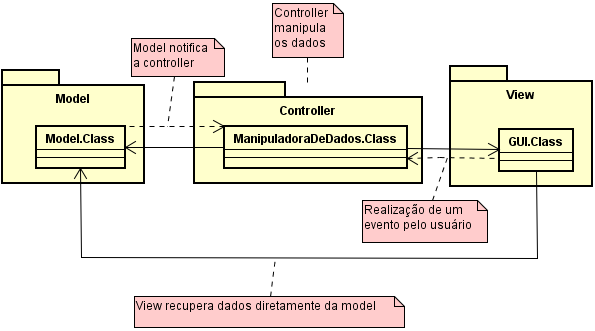
\includegraphics[keepaspectratio=true,scale=0.9]{figuras/DiagramaDeClasseMVC.PNG}
	\caption{Diagrama de classes representando a interação entre os componentes no padrão arquitetural MVC. Adaptado de \cite{durelli2008proposta}.}
	\label{DiagramaDeClasseMVC}
\end{figure}

\pagebreak

A Figura \ref{DiagramaDeSequenciaMVC} é um diagrama de sequência que representa o fluxo dos eventos em um cenário exemplo, no qual a \textit{Controller} interage diretamente com a \textit{Model} e a \textit{View}, sendo que o usuário entra com alguma informação e aguarda o retorno da aplicação. 


\begin{figure}[h!]
	\centering
	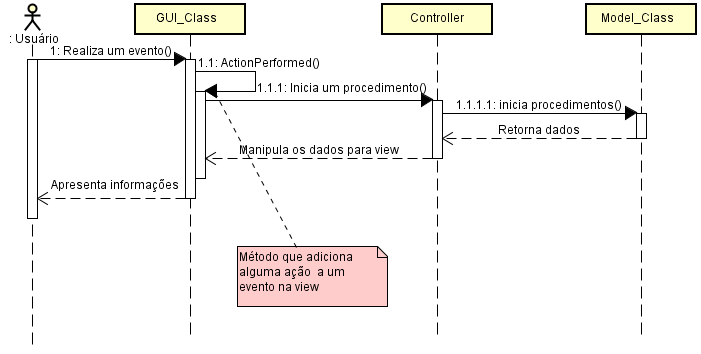
\includegraphics[keepaspectratio=true,scale=0.8]{figuras/DiagramaDeSequenciaMVC.PNG}
	\caption{Diagrama de sequência para o padrão arquitetural MVC. Adaptado de \cite{durelli2008proposta} e \cite{buschmann1996system}.}
	\label{DiagramaDeSequenciaMVC}
\end{figure}

Agora que as principais áreas atreladas ao trabalho foram apresentadas, segue um detalhamento do critério Segurança, também chave para esse trabalho, sendo esse critério tratado como um RNF.


\section{Segurança vista como um RNF}
\label{sec:seguranca}

Tratando a Segurança como um RNF, pode-se entender a mesma como estando associada a vários outros RNFs. Dessa forma, podemos entender os RNFs associados à Segurança como sendo restrições, as quais realizam operacionalizações e satisfazem as metas de segurança, estabelecidas pelos Engenheiros de Requisitos e/ou Engenheiros de Software. Esse conjunto de  RNFs devem expressar de maneira precisa e não ambígua as metas de segurança de uma aplicação, fornecendo uma especificação para alcançar a meta deseja \cite{haley2006framework}.  

Existem variadas definições de Segurança. De forma simplificada, Segurança, no contexto de Segurança da Informação, significa proteger a informação \cite{chung2012non}. O presente trabalho fundamenta-se nos conceitos de \cite{chung2012non} e \cite{sullivan2011web} como base para definir Segurança, orientando-se por três conceitos conhecidos como CIA (\textit{Confidentiality}, \textit{Integrity}, \textit{Availability}) . 

Diante do exposto, para a definição seguindo os fundamentos de \cite{chung2012non}, segurança se baseia em: 

\begin{itemize}
	\item \textbf{Confidencialidade} (do inglês, \textit{Confidenciality}): Proteção da informação para evitar que as informações armazenadas ou transmitidas não sejam vistas ou interpretadas por terceiros, sendo somente o usuário principal e o destinatário. Deve-se prover essa proteção da informação através de algoritmos de criptografia \cite{chung2012non} \cite{silva2007arquitetura}. 
	
	\item \textbf{Integridade} (do inglês, \textit{Integrity}): Proteção contra qualquer tipo de atualização e/ou adulteração não autorizada. Certifica-se que essa proteção seja garantida contra todo tipo de modificação acidental ou maliciosa, garantindo que a informação percorra todo o trajeto entre o usuário principal e um destinatário \cite{chung2012non} \cite{silva2007arquitetura}. 
	
	\item \textbf{Disponibilidade} (do inglês, \textit{Availability}): Proteção contra a interrupção do serviço, no momento em que o usuário principal estiver necessitando da utilização do serviço \cite{chung2012non} \cite{silva2007arquitetura}.
	  
\end{itemize}


O CIA pode ser abstraído em metas flexíveis associadas à Segurança. Logo após, essas metas flexíveis devem ser capturadas e organizadas em um catálogo de Segurança, promovendo um conjunto rico de alternativas e pontos de verificação para se proteger contra possíveis negligencias de pontos relevantes, e para assegurar informações em uma aplicação. Como apresentado na Figura \ref{catalogoSegurancaChung}, abaixo de cada conceito chave de Segurança, existem seus subtipos. 

Apresentados em  verde na Figura \ref{catalogoSegurancaChung}, estão outras características dos requisitos de Segurança, sendo um dos mais relevantes o ``operacional``, que possui como subtipo ``segurança operacional`` referindo-se, diretamente, à Segurança da Informação \cite{chung2012non}.


Os subtipos das “características dos RNFs”, de acordo com \cite{chung2012non}, podem ser “ciclo de vida”, “operacional\footnote[1]{Operação realizada por uma aplicação de software em tempo de execução \cite{chung2012non}.}”, “desenvolvimento\footnote[2]{Estágios de desenvolvimento \cite{chung2012non}.}”, “interna-externa\footnote[3]{Refere-se a confidencialidade dos itens de informação do sistema \cite{chung2012non}.}”, “interna” e “externa”.

\begin{figure}[h!]
	\centering
	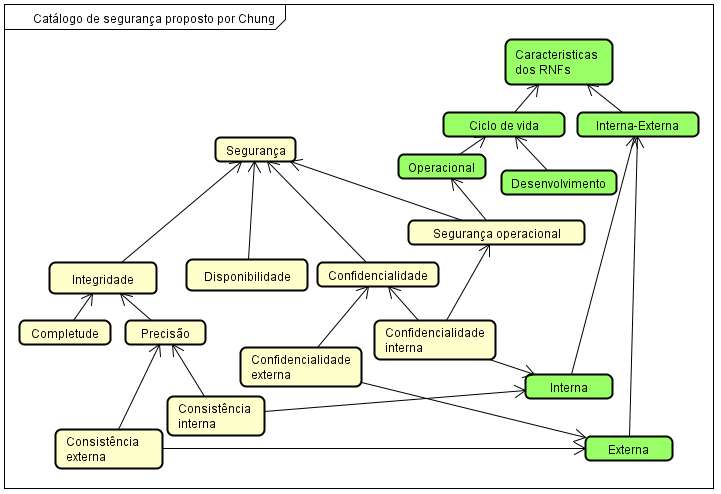
\includegraphics[keepaspectratio=true,scale=0.9]{figuras/catalogoSegurancaChung.PNG}
	\caption{Catálogo de Segurança. Fonte: \cite{chung2012non}.}
	\label{catalogoSegurancaChung}
\end{figure}

É de extrema importância entender os subtipos de cada conceito. Portanto, as subseções a seguir fazem uma breve apresentação sobre os conceitos de Confidencialidade, Integridade e Disponibilidade. 

\subsection{Confidencialidade}
\label{subsec:confidencialidade}

De acordo com \cite{reis10classificaccao}, em Confidencialidade, podem ser definidos conceitos sobre o tipo de Segurança, sendo eles:

\begin{itemize}
	\item \textbf{Irrestrito}: tipo de informação pública; 
	
	\item \textbf{Interna}: tipo de informação que seu acesso deve ser evitado por público externo. Caso este tipo de informação seja disponibilizado, por erro interno ou por ataque malicioso, não causa impacto algum ao mantenedor da informação;
	
	\item \textbf{Confidencial}: tipo de informação interna, a qual, uma vez disponibilizada ao público externo, por erro interno ou ataque malicioso, pode gerar vantagens a concorrentes e, consequentemente, perda de usuários/clientes; 
	
	\item \textbf{Secreta}: tipo de informação interna, restrita a um conjunto específico de usuários, a qual, uma vez disponibilizada tanto ao público externo, quanto ao público interno não definidos, pode causar grandes danos. A integridade dessa informação deve ser mantida a qualquer custo.
\end{itemize} 

A Confidencialidade possui os subtipos “confidencialidade interna” e “confidencialidade externa” conforme ilustra a Figura \ref{catalogoSegurancaChung}.
 

\subsection{Integridade}
\label{subsec:integridade}
 
Integridade pode ser definida através dos conceitos Precisão e Completude, por \cite{chung2012non}, onde: 

\textbf{Precisão}: pode ser entendida como qualquer atributo semântico que fundamenta uma informação \cite{chung2012non}, ou seja, a garantia de que um requisito da informação seja descrito com precisão de acordo com suas especificações; 

\begin{itemize}
	\item \textbf{Propriedade da precisão}: garantir que objetos sejam instanciados da maneira correta; 
	
	\item \textbf{Valor de precisão}: garantir que os valores retornados pelas operações possuam a precisão desejada;
	
	\item \textbf{Precisão de um para um}: Garantir que um único objeto esteja ligado a uma única entidade do domínio. 
	
	\item \textbf{Consistência interna}: garantir que os valores do mundo real sejam correspondentes aos valores do sistema, e
\end{itemize}

\textbf{Completude}: garantir que o RNF esteja completo \cite{chung2012non}. 

\subsection{Disponibilidade}
\label{subsec:disponibilidade}

Um vez introduzidas as áreas de interesse  desse trabalho, bem como o conceito de Segurança sob o ponto de vista de um RNF, cabe ainda comentar sobre o conceito de Personas. Esse conceito foi utilizado no trabalho visando auxiliar na elaboração bem como na evolução do Catálogo de Segurança, considerando diferentes cenários de uso. O conceito de Persona é tratado a seguir, nesse capítulo. Já a aplicação desse conceito nos cenários de uso para elaboração e evolução do catálogo será detalhada no Capítulo \ref{chap:resultadosObtidos} de Resultados Obtidos.

\section{Personas}
\label{sec:personas}

Personas são especificações comportamentais que incorporam as metas e necessidades de usuários, esse conceito foi introduzido para auxiliar os desenvolvedores a entender melhor os usuários diante da necessidade de especificação de um sistema. Personas podem ser aplicadas na Engenharia de Software desde as atividades inerentes à Engenharia de Requisitos, até a entrega do produto propriamente dito \cite{ford2017characterizing}. 

Mais especificamente nesse trabalho, Personas foram utilizadas para levantamento de aspectos chave de segurança, privacidade e outras metas flexíveis de interesse, o que mitigou um pouco as dificuldades enfrentadas no entendimento bem como na especificação dos perfis de usuários compreendidos no escopo dessa pesquisa. Isso viabilizou, dentre outras contribuições, a modelagem de aspectos sociais e psicológicos, promovendo o entendimento dos perfis de usuários, e suas possíveis motivações, as quais permeiam suas ações \cite{ford2017characterizing} \cite{daelaboraccao}. 



Ao longo do processo de construção de uma solução computacional - sob a perspectiva de um produto, tem-se a necessidade de imaginar como esse produto irá funcionar, e como seria possível aplicar esse produto \cite{soegaard2012encyclopedia}. Nesse contexto, se os integrantes de uma equipe de desenvolvimento fizerem uso de Personas, o mesmos serão auxiliados, e terão maiores chances de manter o produto de acordo com os pontos de vista acordados, permitindo maior aderência desse produto às perspectivas dos usuários.Isso é possível, pois se pode imaginar como o produto será utilizado por uma Persona, a qual representa as metas e necessidades de um possível interessado nesse produto. Portanto, a intenção do uso de Personas não é descrever a persona em si, mas sim potencializar a capacidade da equipe no que tange a compreensão do produto, sendo esse idealizado sob diferentes pontos de vista \cite{soegaard2012encyclopedia}.


No presente trabalho, apesar de se reconhecer a relevância do uso do conceito de Personas para mapeamento de aspectos sociais e psicológicos, não foi esse o maior foco. No caso, o uso de Personas contribuiu significativamente para construir o catálogo considerando pontos de vista diferentes, ora com maior olhar em Confiabilidade, ora em Integridade, ora em Disponibilidade, ora focado no Padrão Arquitetural MVC, dentre outras perspectivas. Esse exercício de considerar o catálogo sob diferentes pontos de vista possibilitou um aprofundamento de suas metas flexíveis, e mais ainda, um maior detalhamento das operacionalizações. Operacionalizações representam ações concretas, possíveis de serem de fato alcançadas, implementadas e atendidas pelos especialistas. Uma vez atendidas, propagam-se suas contribuições em atendimento aos aspectos mais abstratos, no caso, as metas flexíveis. Diante dessas colocações, tem-se que o uso de Personas, em cenários de uso variados, contribuiu para a concretização do Catálogo de Segurança elaborado nesse trabalho.


\section{Resumo do Capítulo}

Neste Capítulo, foram abordados os conceitos fundamentais para a construção do Catálogo de Segurança, introduzindo conceitos chave da Engenharia de Requisitos, mais especificamente da Engenharia de Requisitos Orientada à Meta, com foco em metas flexíveis; bem como considerando conceitos chave de Arquitetura de Software, mais precisamente do Padrão Arquitetural MVC.
Dada a relevância do critério de Segurança para o escopo do trabalho, no capítulo, tem-se uma seção dedicada à apresentação desse critério como um RNF. Conforme acordado, Confiabilidade, Integridade e Disponibilidade são metas flexíveis que impactam diretamente em Segurança. Por fim, comentou-se sobre o conceito de Personas, o qual representou um recurso relevante na elaboração bem como na evolução do Catálogo de Segurança sob diferentes pontos de vista, e considerando variados cenários de uso. 
 




